\section{Diseño de la Plataforma}
\thispagestyle{plain}

\vspace{0.5cm}

\Large\scshape
\begin{center}
    \textrm{Diseño de los circuitos principales y auxiliares de la plataforma}
\end{center}
\normalfont
%\normalsize

\divider

Si bien con el análisis del anterior capítulo se pudo conseguir un panorama general del funcionamiento de la plataforma, se presentan otras complejidades a la hora de plasmarlo en un sistema real: se requieren múltiples circuitos auxiliares además de los bloques principales (por ejemplo circuitos de adquisición de señales); aparecen consideraciones de diseño que no existen en el plano teórico; entre otras cuestiones. Este capítulo está dedicado al diseño real de la plataforma completa para luego implementar en una placa de circuito impreso o PCB, teniendo en cuenta estas complicaciones.\\

En la siguiente figura se muestra un diagrama detallado de la plataforma, dónde se presentan todos los distintos bloques funcionales, incluyendo los bloques auxiliares que no se trataron en el análisis del anterior capítulo.\\

\begin{figure}[h]
    \centering
    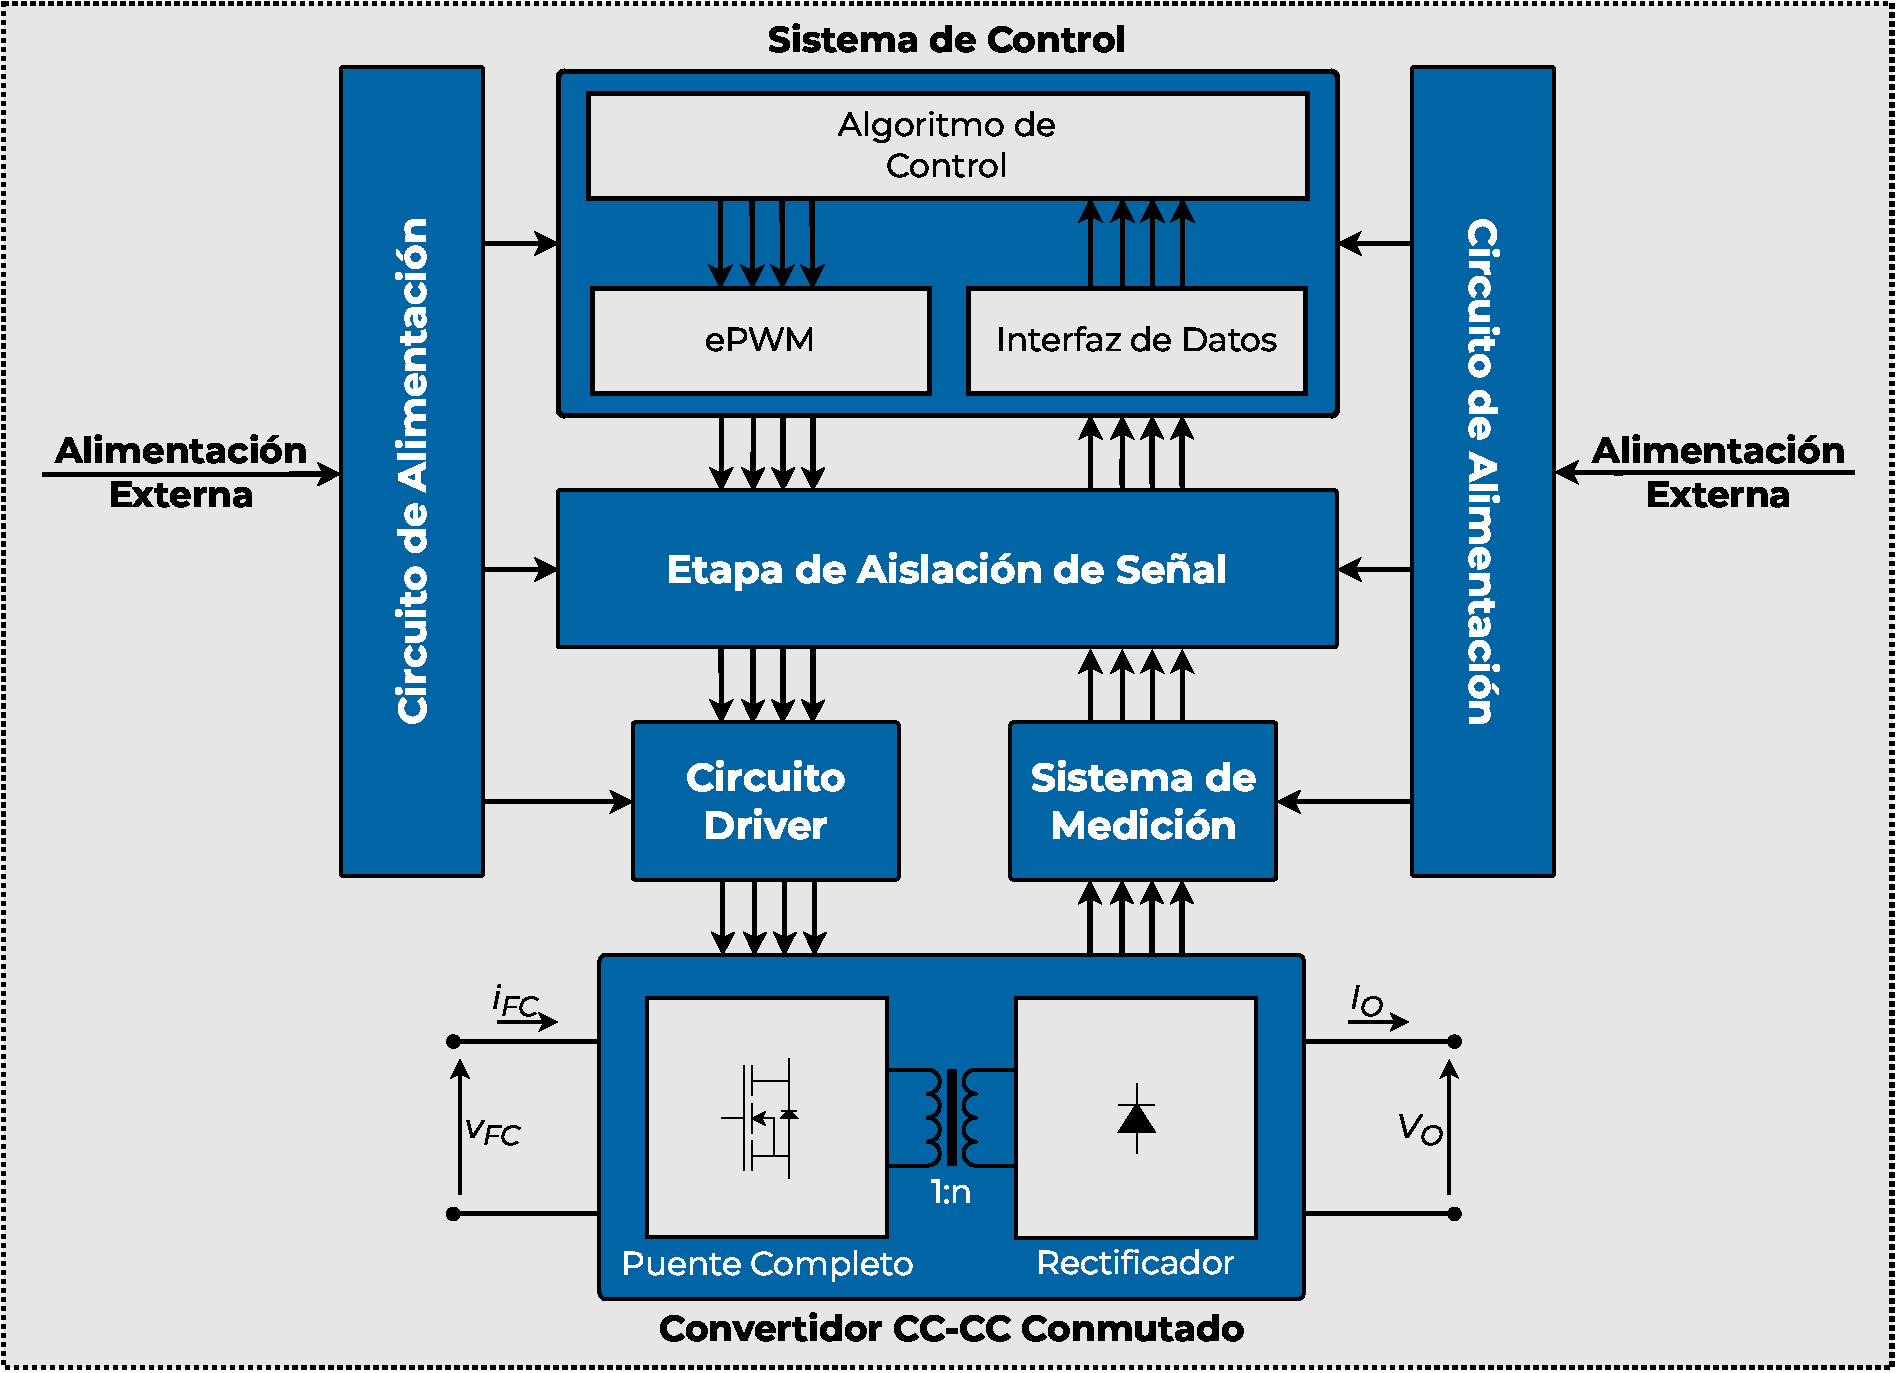
\includegraphics[scale=0.2]{Imagenes/Plataforma Detallada.pdf}
    \caption{Diagrama detallado de la plataforma de evaluación, incluyendo los distintos circuitos auxiliares (Placeholder).}
    \label{diag_detallado}
\end{figure}

Cada uno de estos seis bloques cumplen una función específica que se detalla a continuación:\\

\begin{itemize}
    \item {\SemiBold Convertidor CC-CC Conmutado:} Este es el convertidor de tipo puente completo que se trató en el capítulo anterior. En este capítulo se va a realizar el dimensionamiento de todos sus componentes teniendo en cuenta sus especificaciones. 
    \item {\SemiBold Circuito \textit{Driver}:} Este circuito se encarga de entregar la corriente y tensión necesaria para disparar los transistores de potencia y conmutarlos correctamente.
    \item {\SemiBold Sistema de Medición:} Este bloque contiene todos los circuitos y componentes necesarios para realizar las mediciones de todos los parámetros de interés de la plataforma. Esto incluye, además de sensores, los circuitos de acondicionamiento de señal donde se requieran.
    \item {\SemiBold Etapa de Aislación:} Esta etapa se encarga de generar una barrera de aislación eléctrica entre los componentes de potencia y los componentes de señal del circuito.
    \item {\SemiBold Sistema de Control:} Este es el bloque de control que se explicó en el anterior capítulo. Obtiene información de distintos parámetros por medio del sistema de medición, y ejerce la acción de control disparando las llaves mediante el driver.
    \item {\SemiBold Circuito de Alimentación:} Es el circuito que se encarga de proveer las corrientes y tensiones necesarias para los componentes que requieren alguna alimentación externa para funcionar (por ejemplo el controlador digital de señales).\\
\end{itemize}

A lo largo de este capítulo se va a tratar uno por uno el diseño de los circuitos que componen a cada uno de los bloques, utilizando múltiples diseños como referencia (ya sean de otros trabajos de investigación o diseños sugeridos de los propios fabricantes). Se van a eligir y dimensionanar los componentes que forman parte de ellos, hasta obtener un esquemático circuital detallado de la plataforma experimental de evaluación completa.\\

Pero antes de comenzar con el primer bloque, se van a plantear algunas consideraciones y criterios generales que se van a utilizar para la selección de todos los componentes y diseño de todos circuitos de la plataforma.\\

\subsection{Consideraciones Generales}

\subsubsection{Aislación de Tierras}

En toda la plataforma se va a trabajar con tres puestas a tierra distintas y aisladas entre sí: $GND_1$ es la tierra del primario del convertidor, $GND_2$ es la tierra del secundario del convertidor, y $GND_D$ es la tierra de las partes de señal y digitales, como los sensores y el DSC.\\

Esto, si bien agrega una mayor complejidad al diseño, es ventajoso por múltiples razones. Primero, evita la generación de interferencia de modo común entre las tierras del convertidor ($GND_1$ y $GND_2$) que manejan altas corrientes y por lo tanto son más ruidosas; y la tierra de señal $GND_D$ de más bajas corrientes que es más sensible al ruido. Además, dadas las altas corrientes del convertidor, esta separación permite la protección de los circuitos de señal ante picos de corriente y tensión inesperados en la parte de potencia.\\

Es por estas razones que además de la tierra, también los circuitos de señal y potencia se encuentran separados por la etapa de aislación entre potencia y señal. Adicionalmente, las fuentes de alimentación externas se encuentran separadas para los componentes de potencia y señal, manteniendo la aislación deseada.\\

\subsubsection{Selección de Componentes}

En líneas generales, a la hora de elegir un circuito para el diseño de los distintos bloques, si es posible se trata de elegir una solución más integrada (es decir utilizar un circuito integrado que haga esta tarea en vez de diseñar un circuito discreto). Esto simplifica los circuitos y disminuye la cantidad de componentes necesarios a la hora de implementarlos. Además, al estar toda la solución integrada, el rendimiento es más predecible y se encuentra acotado a los parámetros dados por el fabricante del circuito integrado.\\

En todos los casos, se utilizan como guía para el diseño de todas las partes los parámetros de rendimiento y las recomendaciones de diseño especificadas en las hojas de datos  y notas de aplicación de los fabricantes de cada circuito integrado.\\

\subsubsection{Herramientas de Software}

\paragraph{Software EDA}

Para realizar el diseño de todos los esquemas circuitales del sistema, y luego plasmarlos a una placa de circuito impreso se debe utilizar un herramienta de automatización de diseño electrónico o EDA (del inglés \textit{Electronic Design Automation}). Existe una gran variedad de programas que cumplen este propósito, estando entre los más conocidos el \textit{Altium Designer} de \textit{Altium}, el \textit{EAGLE} de \textit{Autodesk}, el \textit{KiCad} y el \textit{Proteus Design Suite} de \textit{Labcenter Electronics}.\\

Para este proyecto se eligió utilizar la plataforma {\Medium KiCad} (que se encuentra en la versión 6.0.7 al momento de escribir este informe), una suite de software libre, gratuita y de código abierto que incluye todas la funcionalidades necesarias para el diseño electrónico. Cuenta con herramientas de captura de esquemático, diseño de PCB, simulación mediante SPICE o Ngspice, visualización de archivos de fabricación y cálculos de diseño de PCB.\\

\begin{figure}[h]
    \centering
    
\includegraphics[scale=0.6]{Imagenes/KiCad.pdf}
    \caption{Logotipo de la plataforma KiCad EDA.}
    \label{logo_kicad}
\end{figure}

El programa también cuenta con una extensa biblioteca de componentes y \textit{footprints} (son las \quotes{huellas} de los componentes en en el circuito impreso) y la capacidad de crear o importar bilbiotecas. Además tiene la capacidad de generar archivos de fabricación, modelos tridimensionales de la PCB y una \textit{bill of materials} (lista de componentes).\\

\paragraph{Software de Simulación}

Para todo lo que se refiere a la simualción de la plataforma; más particularmente las simulaciones del funcionamiento del convertidor CC-CC para su comprensión, estudio, diseño y dimensionamiento; se utilizó la herramienta {\Medium\textit{Simulink}} dentro de la suite de software de \textit{MATLAB-Simulink}.\\

\begin{figure}[h]
    \centering
    
\includegraphics[scale=0.08]{Imagenes/Simulink.png}
    \caption{Logotipo de la plataforma de simulación Simulink.}
    \label{logo_simulink}
\end{figure}

Específicamente, para simulaciones circuitales se hizo uso de el paquete \textit{Simscape Electrical} dentro de Simulink, que permite trabajar con tensiones y corrientes, a diferencia de las herramientas estándar que trabajan con diagramas de bloques.\\

\paragraph{Otras Herramientas}

Adicionalmente, para llevar un control de versiones completo del diseño de la plataforma sobre el que se trabaja, además de mantener un historial completo de todos los cambios, se trabajó con la herramienta de software de control de versiones {\Medium\textit{Git}}.\\

\begin{figure}[h]
    \centering
    
\includegraphics[scale=0.6]{Imagenes/Git.pdf}
    \caption{Logotipo del software de control de versiones Git.}
    \label{logo_git}
\end{figure}

Con este software se crea un \textit{repositorio} donde se almacenan los archivos que se quiere controlar, manteniendo un control de la historia de cada uno de los archivos del repositorio. Para mantener los archivos sincronizados entre varias computadoras y mantener copias de seguridad, se utiliza adicionalmente la plataforma web {\Medium\textit{GitHub}} para hostear el repositorio en la nube, manteniendo una copia segura que se puede copiar a cualquier computadora.\\

\newpage

\subsection{Convertidor CC-CC Conmutado}

Para llevar a cabo el diseño del convertidor, primero debemos establecer los objetivos de rendimiento del mismo (como por ejemplo, la tensión que debe tener a la salida). Con estos valores establecidos, y junto con otras consideraciones del diseño, se van a obtener todos los parámetros que definen al convertidor, como las llaves y diodos a utilizar, tamaño de capacitores e inductores, etc.\\

\begin{figure}[h]
    \centering
    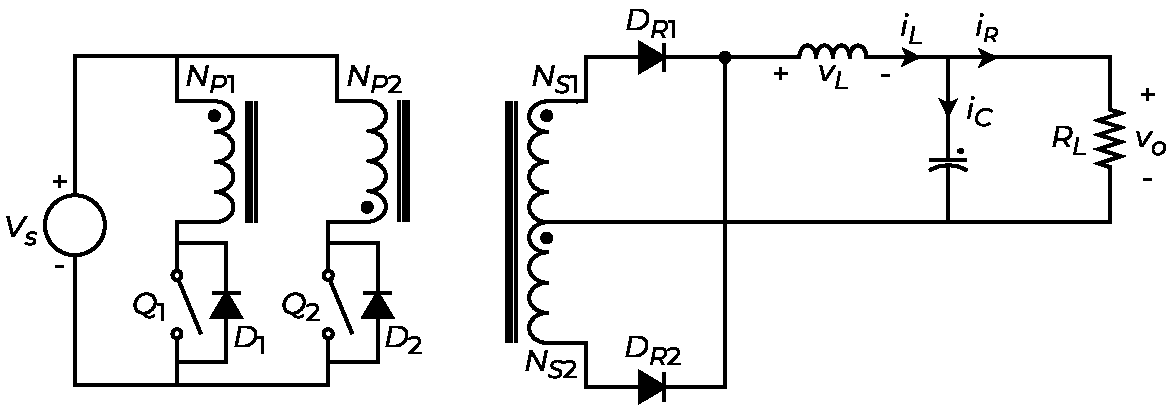
\includegraphics[scale=0.6]{Imagenes/Push-Pull.pdf}
    \caption{Diagrama del convertidor CC-CC de tipo puente completo a utilizar, con todos sus componentes (Placeholder).}
    \label{puente_completo}
\end{figure}

\subsubsection{Especificaciones de Diseño}

La plataforma experimental va a ser utilizada para la evaluación de un módulo de pilas de combustible de \SI[]{300}[]{\watt} de potencia nominal, entregando \SI[]{36}[]{\volt} a \SI[]{8.3}[]{\ampere} de corriente. La tensión de salida varía desde \SI[]{65}[]{\volt} a circuito abierto hasta \SI[]{30}[]{\volt} para la máxima corriente de \SI[]{9.5}[]{\ampere}.\textsuperscript{\cite{HSeriesBrochure}}\\

Esta potencia debe ser transferida por el convertidor hacia la carga variable a la salida, que emula distintas condiciones de carga del bus común de corriente continua de \SI[]{75}[]{\volt} fijos. Dada la potencia de \SI[]{300}[]{\watt}, y si la tensión de salida es la del bus común, entonces el sistema debe soportar una corriente de salida máxima de alrededor de \SI[]{4}[]{\ampere}. Adicionalmente, las llaves del primario van a conmutar a una frecuencia de conmutación de \SI[]{20}[]{\kilo\hertz}, y se debe reducir lo más posible las pérdidas de energía por conmutación, para darle una mayor escalabilidad al diseño.\\

\begin{itemize}
    \item {\SemiBold Potencia nominal \textit{P\textsubscript{N}}:}\quad\SI[]{300}[]{\watt}
    \item {\SemiBold Tensión de salida \textit{v\textsubscript{o}}:}\quad\SI[]{75}[]{\volt}
    \item {\SemiBold Corriente de salida \textit{i\textsubscript{o}}:}\quad\SI[]{4}[]{\ampere}
    \item {\SemiBold Tensión de entrada \textit{v\textsubscript{FC}}:}\quad\SI[]{65}[]{\volt}\textsubscript{máx} , \SI[]{30}[]{\volt}\textsubscript{mín}
    \item {\SemiBold Corriente de entrada \textit{i\textsubscript{FC}}:}\quad\SI[]{9.5}[]{\ampere}
    \item {\SemiBold Frecuencia de conmutación \textit{f\textsubscript{s}}:}\quad\SI[]{20}[]{\kilo\hertz}\\
\end{itemize}

Entonces, con todas estas características quedan definidas las especificaciones necesarias para comenzar la selección y dimensionamiento de componentes del convertidor. Se va a tratar el diseño de cada componente uno por uno, comenzando por los cuatro transistores de potencia que se encargan de la conmutación.\\

\subsubsection{Selección de Llaves}

Las cuatro llaves ideales que conforman el circuito puente del lado primario son implementadas por algún dispositivo electrónico de tres terminales (los dos terminales de potencia, y un tercer terminal de control con el que se comanda la conmutación de la llave). Existen dentro de estas llaves dos categorías distintas: las \textit{llaves semicontroladas}, donde la llave no se puede controlar completamente (por ejemplo se puede comandar el cierre pero no la apertura) y las \textit{llaves completamente controladas} que, como su nombre dice, pueden ser cerradas y abiertas mediante su tercer terminal.\\

En nuestro caso, la topología de puente completo exige la apertura y cierre de las cuatro llaves a la frecuencia de conmutación, por lo que se requieren {\Medium llaves completamente controladas}, dentro de las cuales se pueden elegir una serie de transistores o tiristores.\\

\paragraph{Tecnologías de Transistores}

En nuestro caso, nos vamos a enfocar únicamente en los tres tipos distintos de transistores de potencia, evaluandolos para su uso en la plataforma: el transistor bipolar o BJT (\textit{Bipolar Junction Transistor}), el transistor IGBT (\textit{Insulated-Gate Bipolar Transistor}) y el transistor de efecto de campo o MOSFET (\textit{Metal-Oxide-Semiconductor Field-Effect Transistor}).\\

\subparagraph{Transistor Bipolar}

El transistor bipolar de la figura \ref{bjt} cuenta con su terminal de control, la \textit{base} (B), y sus dos terminales de potencia, el \textit{colector} (C) y \textit{emisor} (E). Este dispositivo se controla mediante la inyección de corriente por la base, por lo que se puede decir que es una llave controlada por corriente.\\

\begin{figure}[h]
    \centering
    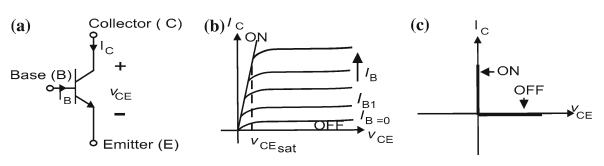
\includegraphics[scale=0.6]{Imagenes/BJT.png}
    \caption{El transistor bipolar (a) su símbolo eléctrico, (b) su curva característica, (c) su curva como llave ideal.}
    \label{bjt}
\end{figure}

Su funcionamiento viene dado por las curvas de corriente de colector $I_C$ contra tensión colector-emisor $V_{CE}$ en el primer cuadrante. El transistor se encuentra en su estado apagado (región de corte) en el área debajo de la curva de corriente de base $I_B$ nula; mientras que se encuentra encendido (región de saturación) en el área donde la tensión $V_{CE}$ es menor a la tensión de saturación ($V_{CE} \leq {V_{CE}}_{sat}$).\\

Hoy en día, los BJT rara vez son utilizados como llaves de potencia, ya que las otras dos tecnologías tienen grandes ventajas frente a este tipo de dispositivo. Primero, al ser un dispositivo controlado por corriente, estos transistores pierden mucha energía de forma disipativa al ser conmutados. Además, al ser un dispositivo de portadores minoritarios, su tiempo de conmutación se ve afectado, cayendo en el orden de los \unit[]{\micro\second}. Sin embargo, como ventaja tienen su baja impedancia de salida, lo que les da una muy baja pérdida de conducción.\textsuperscript{\cite{PotenciaHart}\cite{PowerElecRenewableEnergySystems}}\\

\subparagraph{MOSFET}

El MOSFET de la figura \ref{mosfet} tiene al \textit{gate} (G) como terminal de control, y los terminales de \textit{drain} (D) y \textit{source} (S) como terminales de potencia. Este transistor se controla mediante la variación de la tensión gate-source $V_{GS}$, por lo que, a diferencia del BJT, es un dispositivo controlado por tensión.\\

\begin{figure}[h]
    \centering
    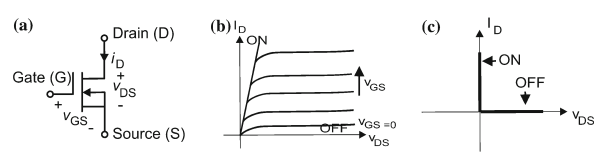
\includegraphics[scale=0.6]{Imagenes/MOSFET.png}
    \caption{El MOSFET (a) su símbolo eléctrico, (b) su curva característica, (c) su curva como llave ideal.}
    \label{mosfet}
\end{figure}

Su funcionamiento es caracterizado por las curvas de corriente de drain $I_D$ versus tensión drain-source $V_{DS}$ en el primer cuadrante. Para encontrarse en estado apagado o región de corte, la tensión de control $V_{GS}$ debe ser menor a una tensión umbral o \textit{threshold} $v_T$ que depende del dispositivo (esto corresponde a la región debajo de la marca OFF en la figura). Cuando la tensión de control supera este umbral, el dispostivo entra en conducción, con una resistencia drain-source ${R_{DS}}_{on}$ baja de orden de \unit[]{\milli\ohm}.\\

Los MOSFET tienen varias características que los hacen deseables como interruptores electrónicos de potencia: al ser controlados por tensión, la pérdida disipativa de potencia para la conmutación es muy baja; como el dispositivo trabaja con portadores mayoritarios, su velocidad de conmutación es muy rápida, con tiempos de conmutación en el orden de los \unit[]{\nano\second}; y tienen una alta impedancia de entrada. Además, por su construcción, tienen un diodo antiparalelo incluido entre D y S, cosa que es deseable para muchas topologías de convertidores.\\

Sin embargo, tienen como desventaja una limitación en tensión y corriente, ya que no soportan corrientes que excedan los \SI[]{200}[]{\ampere} ni tensiones por encima de \SI[]{1}[]{\kilo\volt}; además de tener una elevada impedancia de salida, generando pérdidas de conducción.\textsuperscript{\cite{PotenciaHart}\cite{PowerElecRenewableEnergySystems}}\\

\subparagraph{IGBT}

Los transistores del tipo IGBT podrían ser considerados como un híbrido entre las dos tecnologías anteriores, combinando las ventajas de ambos. Este dispositivo tiene un terminal de control llamado gate (G) al igual que el MOSFET, y dos terminales de potencia, el colector (C) y emisor (E), al igual que el BJT. Se controla mediante la tensión gate-emisor $V_{GE}$, por lo que es controlado por tensión al igual que el MOSFET.\\

\begin{figure}[h]
    \centering
    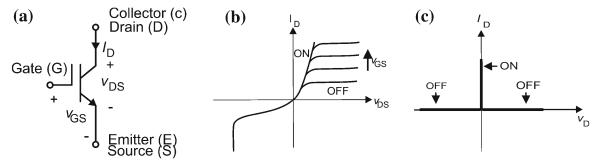
\includegraphics[scale=0.6]{Imagenes/IGBT.png}
    \caption{El IGBT (a) su símbolo eléctrico, (b) su curva característica, (c) su curva como llave ideal.}
    \label{igbt}
\end{figure}

Se caracteriza por la curva de corriente de colector $I_C$ contra tensión gate-emisor $V_{GE}$ de la figura \ref{igbt}, y a diferencia de los anteriores dos transistores, opera en los cuadrantes primero y segundo, es decir que puede bloquear tensión bidireccionalmente y conducir corriente de forma unidireccional.\\

Este transistor combina las ventajas de los BJT y los MOSFET, es decir que tiene una alta impedancia de entrada como el MOSFET, disminuyendo las pérdidas disipativas de la conmutación; una baja impedancia de salida como el BJT, disminuyendo las pérdidas de conducción; y soporta muy altas tensiones, por encima de \SI[]{1}[]{\kilo\volt}, y corrientes mayores a \SI[]{500}[]{\ampere}. Sin embargo, si bien su velocidad de conmutación es superior a la del transistor bipolar, pero no alcanza los cortos tiempos del orden de \unit[]{\nano\second} de los MOSFET, además de ser la tecnología más costosa dentro de las presentadas.\textsuperscript{\cite{PotenciaHart}\cite{PowerElecRenewableEnergySystems}}\\

\paragraph{Selección de MOSFET}

Como las llaves de la plataforma de evaluación nunca excederán los \SI[]{15}[]{\ampere}, y la tensión sobre las llaves no puede superar los \SI[]{70}[]{\volt}, los transistores del tipo MOSFET son la elección más lógica. Sus límites de tensión y corriente están muy por encima de los requierimientos de este diseño, tienen la velocidad de conmutación más rápida y son más económicos que los IGBT. SI bien sus pérdidas de conducción son elevadas, para aplicaciones de relativamente baja potencia como la de este proyecto, se pueden conseguir modelos con muy bajara resistencia de salida ${R_{DS}}_{on}$, mitigando la mayor desventaja de esta tecnología.\\

Entonces, habiendo seleccionado una tecnología de llave, ahora debemos elegir un modelo particular de MOSFET que satisfaga los parámetros necesarios para ser utilizado en el puente de transistores del convertidor. Las características que debe cumplir son:\\

\begin{itemize}
    \item Tensión drain-source $V_{DS} > \SI[]{65}[]{\volt}$, dado que cada transistor debe soportar tensión igual a ${v_{FC}}_{max}$.
    \item Corriente de drain continua $I_D > \SI[]{10}[]{\ampere}$, que es la corriente máxima que es capaz de entregar el modulo de pila de combustible.
    \item Potencia de disipación $P_D > \SI[]{75}[]{\watt}$, ya que la potencia nominal de \SI[]{300}[]{\watt} se distribuye entre las cuatro llaves.
    \item Tiempo de \textit{rise} $t_r$ y \textit{fall} $t_f$ mucho menor al tiempo de un período $T_s = 1/f_s = \SI[]{50}[]{\micro\second}$.
    \item Resistencia de salida ${R_{DS}}_{on}$ lo más baja posible.
    \item Encapsulado \textit{through-hole} capaz de manejar altas disipaciones de potencia.\\
\end{itemize}

Con esto en cuenta, se debe buscar en catálogos y leer especificaciones en hojas de datos para elegir un modelo que cumpla con estas características. Consultando en comerciantes locales y en páginas internacionales como Mouser o DigiKey, se llegó a la familia IRFP de MOSFETs de potencia, con una amplia selección de corrientes y tensiones máximas.\\

Particularmente, se eligió el modelo {\Medium IRFP150N de International Rectifier} (hoy en día parte de Infineon Technologies), cuyas especificaciones se muestran en la siguiente tabla. Estos dispositivos se eligieron por su bajo tiempo de conmutación y resistencia de salida, además fue un factor adicional la disponibilidad de los mismos en el instituto, eliminando la necesidad de comprarlos.\\

\setlength{\tabcolsep}{7pt}
\renewcommand{\arraystretch}{1.5}
\begin{table}[h]
\begin{center}
    \begin{tabular}{lrrrrrrr}
    {\SemiBold Modelo} & $\mathbf{V_{DS}}$ [\unit{\volt}] & $\mathbf{I_D}$ [\unit{\ampere}] & $\mathbf{P_D}$ [\unit{\watt}] & $\mathbf{{R_{DS}}_{on}}$ [\unit{\milli\ohm}] & $\mathbf{t_{on}}$ [\unit{\nano\second}] & $\mathbf{t_{off}}$ [\unit{\nano\second}] & $\mathbf{{V_{GS}}_{th}}$ [\unit{\volt}]\\
    \hline
    IRFP150N & \num{100} & \num{42} & \num{160} & \num{36} & \num{67} & \num{85} & \num{4}
    \end{tabular}
    \caption{Especificaciones del MOSFET de potencia IRFP150N de International Rectifier.\textsuperscript{\cite{DatasheetIRFP150}}}
    \label{tabla:IRFP150}
\end{center}
\end{table}

Donde $V_{DS}$ es la tensión de ruptura drain-source, $I_D$ es la máxima corriente continua de drain, $P_D$ es la máxima disipación de potencia, ${R_{DS}}_{on}$ la resistencia drain-source en estado encendido, $t_{on}$ y $t_{off}$ el tiempo de encendido y apagado, y ${V_{GS}}_{th}$ la tensión umbral para el encendido del transistor.\\

Este transistor es un nMOSFET (canal N) de enriquecimiento de tecnología HEXFET, que tiene incluido en su interior el diodo antiparalelo necesario para la topología de convertidor en uso. Como se puede ver en las especificaciones, cumple con todos nuestros requerimientos: soporta tensiones, corrientes y potencias muy por encima de las requeridas (dando un buen margen de seguridad); una resistencia de conducción muy baja, resultando en pérdidas de menos de \SI[]{0.5}[]{\watt} en cada transistor para \SI[]{10}[]{\ampere} de corriente; y tiempos de encendido y apagado más de cien veces menor al $T_s$ de \SI[]{50}[]{\micro\second}.\\

\begin{figure}[h]
    \centering
    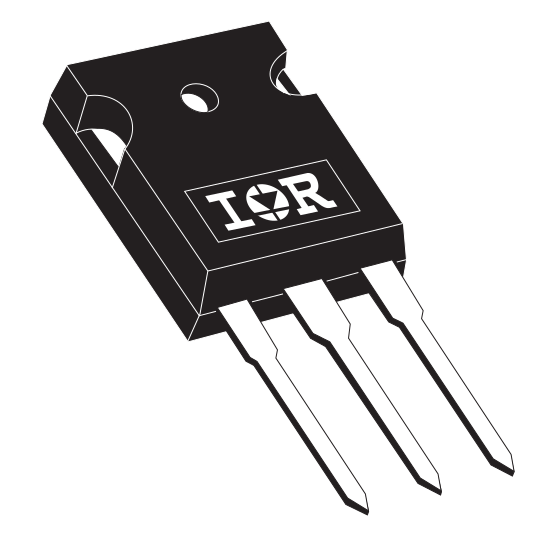
\includegraphics[scale=0.15]{Imagenes/IRFP150-TO247AC.png}
    \caption{MOSFET IRFP150N con su encapsulado THT de potencia tipo TO-247AC.}
    \label{irfp150}
\end{figure}

El encapsulado es del tipo TO-247AC, visible en la figura \ref{irfp150}. Este es un encapsulado through-hole o THT utilizado para dispositivos de alta disipación de potencia, por su tamaño y su superficie metálica que facilita la utilización de un disipador para mantener la temperatura bajo control.\\

\subsubsection{Transformador}

\lipsum[3]\\

\lipsum[4]\\

\subsubsection{Selección de Diodos Rectificadores}

Ahora debemos seleccionar los cuatro diodos que conforman el rectificador de puente completo en el secundario del convertidor. Al igual que los transistores de la sección anterior, estos deben ser diodos de potencia capaces de manejar la potencia de \SI[]{300}[]{\watt} que circulará a través de ellos. Se enumeran a continuación los requerimientos que deben cumplir los diodos seleccionados:\\

\begin{itemize}
    \item Tensión inversa $V_R > \SI[]{150}[]{\volt}$.
    \item Corriente directa $I_F > \SI[]{4.5}[]{\ampere}$.
    \item Tiempo de recuperación de inversa $t_{rr}$ mucho menor al período de conmutación $T_s$ de \SI[]{50}[]{\micro\second}.
    \item Encapsulado THT capaz de manejar altas disipaciones de potencia.\\
\end{itemize}

Con estas especificaciones en cuenta, se eligieron los diodos ultrafast recovery de la serie MUR, particularmente el modelo MUR860 por su corto tiempo de recuperación inversa, baja caída de tensión en conducción y alta tensión inversa máxima. Se detallan sus especificaciones importantes en el siguiente cuadro.\\

\setlength{\tabcolsep}{7pt}
\renewcommand{\arraystretch}{1.5}
\begin{table}[h]
\begin{center}
    \begin{tabular}{llrrrr}
    {\SemiBold Fabricante} & {\SemiBold Modelo} & $\mathbf{V_{RRM}}$ [\unit{\volt}] & $\mathbf{I_{F(AV)}}$ [\unit{\ampere}] & $\mathbf{V_F}$ [\unit{\volt}] & $\mathbf{t_{rr}}$ [\unit{\nano\second}]\\
    \hline
    ON Semiconductor & MUR860 & \num{600} & \num{8} & \num{1.5} & \num{60}\\
    \end{tabular}
    \caption{Especificaciones del diodo rectificador ultrafast recovery MUR860 de ON Semiconductor.\textsuperscript{\cite{MUR860}}}
    \label{tabla:MUR860}
\end{center}
\end{table}

Donde $V_{RRM}$ es la máxima tensión inversa repetitiva, $I_{F(AV)}$ es la máxima corriente rectificada promedio, $V_F$ es la tensión directa instantánea y $t_{rr}$ el máximo tiempo de recuperación inversa.\\

Estos son diodos rectificadores de potencia de la gama ultrafast recovery, pensados para aplicaciones en fuentes de corriente continua conmutadas, como es el caso de este convertidor. Como se ve en el cuadro \ref{tabla:MUR860}, este diodo tiene una tensión inversa máxima muy por encima de los requerimientos, al igual que la máxima corriente directa, que es cerca del doble de lo requerido, dando buenos márgenes de seguridad. Su tiempo de recuperación es similar a los tiempos de conmutación de los transistores IRFP150N de la tabla \ref{tabla:MUR860}, y su caída de tensión en directa de \SI[]{1.5}[]{\volt} es adecuadamente baja.\\

\begin{figure}[h]
    \centering
    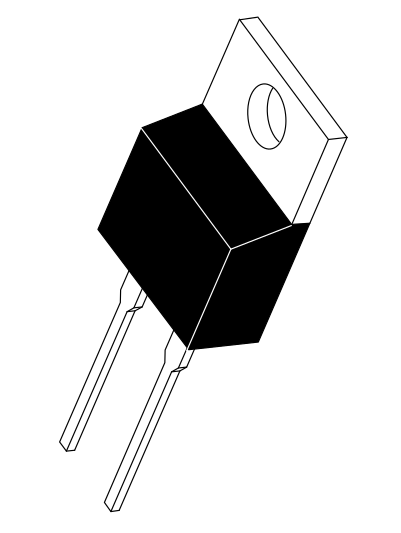
\includegraphics[scale=0.18]{Imagenes/MUR860.png}
    \caption{Diodo rectificador MUR860 con su encapsulado THT de potencia tipo TO-220AC.}
    \label{mur860}
\end{figure}

Se observa este diodo en su encapsulado THT de potencia tipo TO-220AC en la figura \ref{mur860}. Al igual que el encapsulado de los transistores IRFP150N, el TO-220AC posee una superficie metálica en contacto directo con el semiconductor interno que facilita la transferencia de calor hacia un disipador metálico.\\

\subsubsection{Inductor de Salida}

\lipsum[5]\\

\lipsum[6]\\

\subsubsection{Capacitores de Filtro}

\lipsum[7]\\

\lipsum[8]\\

\newpage

\subsection{Circuito Driver}

Como se explicó más arriba, para excitar un transistor MOSFET y encenderlo, es necesario mantener una tensión $V_{GS}$ entre gate y source mayor a una tensión umbral dependiente del modelo. En nuestro caso, esta tensión umbral del IRFP150N es de \SI[]{4}[]{\volt}, como se ve en la tabla \ref{tabla:IRFP150}. Entonces, se debe diseñar algún circuito que sea capaz de proveer estos pulsos de tensión al gate de cada transistor, entregando también la corriente necesaria para cargar y descargar sus capacitancias de gate suficientemente rápido (llamadas corrientes de \textit{source} y \textit{sink}).\\

Este es el llamado {\Medium circuito \textit{driver}} o {\Medium circuito de excitación} y debe existir uno para cada uno de los cuatro transistores del puente. Ahora debemos establecer algunos requerimientos que debe cumplir el circuito:\\

\begin{itemize}
    \item Tensión de operación mayor a \SI[]{100}[]{\volt}, por encima de la máxima tensión de la pila de combustible.
    \item Tiempos de encendido y apagado mucho menores al período $T_s$ de \SI[]{50}[]{\micro\second} de la excitación.
    \item Corrientes de sink y source mayores a \SI[]{2}[]{\ampere} para cargar rápidamente las capacitancias de los transistores, calculado según la nota de aplicación de \cite{SinkSourceCurrent}.
    \item Se busca utilizar una solución integrada, ya que suelen ser más compactas y sencillas.
    \item Es deseable el uso de componentes de montaje superficial o SMD.\\
\end{itemize}

Con estos datos vamos a seleccionar y diseñar un circuito de excitación y explicar brevemente el funcionamiento de todas sus partes.\\

\subsubsection{Selección y Diseño}

Existen diversos tipos de soluciones integradas para circuitos de excitación de transistores MOSFET. Se pueden encontrar circuitos de uno o múltiples canales; existen circuitos que incluyen una aislación entre las entradas y salidas; entre otras funcionalidades. También se consiguen con distintas funciones de seguridad y protección, como el \textit{dead-time}, que permite forzar un tiempo fijo entre la activación de dos transistores de la misma rama, evitando situaciones de cortocircuito; y el \textit{undervoltage lockout} (UVLO), que evita daños por condiciones de baja tensión.\\

Entre todas las opciones, originalmente se había decidido por el modelo UCC21540 de Texas Instruments, un driver de doble canal, con aislación incluida, funcionalidades de dead-time y UVLO, alta capacidad de corriente y un encapsulado SMD de tipo SOIC-16.\\

Sin embargo, este dispositivo no se pudo obtener por falta de disponibilidad, por lo que se tuvo que buscar una alternativa de características similares que esté en disponibilidad. Se terminó decidiendo por el integrado {\Medium 2ED21834-S06J de Infineon Technologies}, cuyas especificaciones básicas se muestran a continuación.\\

\setlength{\tabcolsep}{7pt}
\renewcommand{\arraystretch}{1.5}
\begin{table}[h]
\begin{center}
    \begin{tabular}{llrrrr}
    {\SemiBold Fabricante} & {\SemiBold Modelo} & $\mathbf{V_S}$ [\unit{\volt}] & $\mathbf{I_{OH}/\mathbf{I_{OL}}}$ [\unit{\ampere}] & $\mathbf{t_{on}}/\mathbf{t_{off}}$ [\unit{\nano\second}] & $\mathbf{V_{cc}}$ [\unit{\volt}]\\
    \hline
    \makecell[l]{Infineon \\ Technologies} & 2ED21834-S06J & \num{650} & \num{2.5} & \num{200} & \num{10}-\num{20}
    \end{tabular}
    \caption{Especificaciones del driver modelo 2ED21834-S06J de Infineon Technologies.\textsuperscript{\cite{DatasheetDriver}}}
    \label{tabla:driver}
\end{center}
\end{table}

Donde $V_S$ es la máxima tensión común de operación, $I_{OH}$ e $I_{OL}$ son las corrientes máximas de source y sink, $t_{on}$ y $t_{off}$ son los tiempos de encendido y apagado, y $V_{cc}$ es el rango de tensiones de alimentación.\\ 

El 2ED21834-S06J es un driver de doble canal para medios puentes de transistores de tipo MOSFET e IGBT, con diodo y resistencia de bootstrap incluidos además de funcionalidad de dead-time y UVLO para circuitos del lado bajo y alto, todo contenido en un encapsulado SMD de catorce pines del tipo DSO-14 (figura \ref{encapsulado_driver}). Sus corrientes sink y source de \SI[]{2.5}[]{\ampere} superan la corriente necesaria calculada para los IRFP150N de la tabla \ref{tabla:IRFP150}, su tensión de operación se encuentra cómodamente por encima de la tensión de operación del primario del convertidor, además de tener muy bajos tiempos de conmutación.\\

\begin{figure}[h]
    \centering
    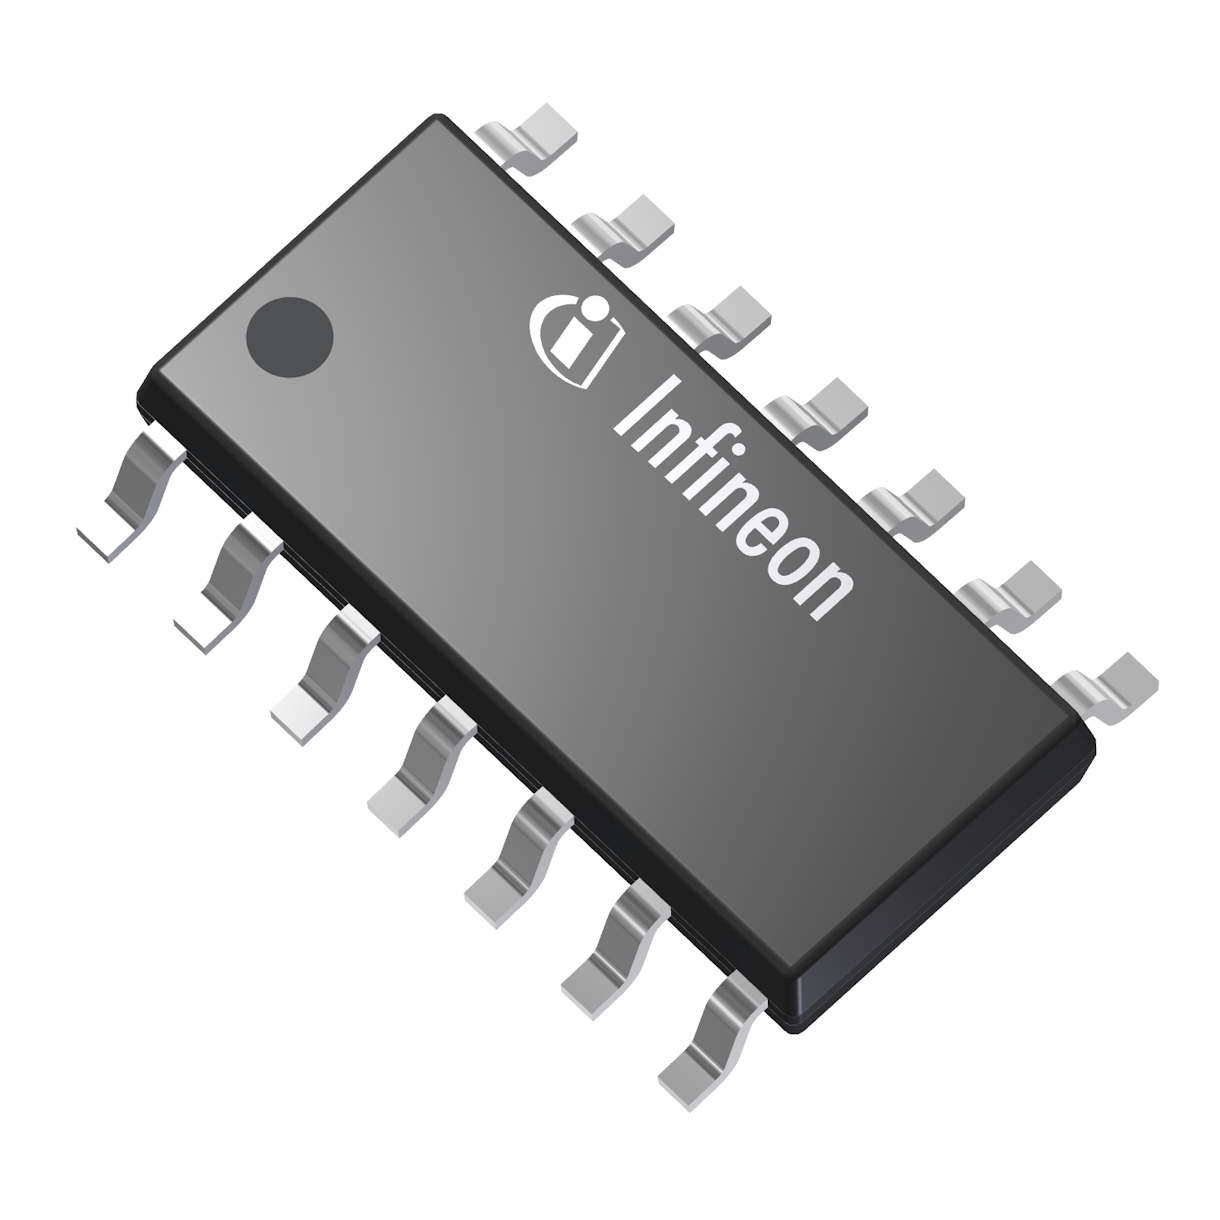
\includegraphics[scale=0.07]{Imagenes/Driver DSO-14.png}
    \caption{Driver 2ED21834-S06J con su encapsulado SMD tipo DSO-14.}
    \label{encapsulado_driver}
\end{figure}

En nuestro caso, se deben utilizar dos de estos dispositivos, uno para cada columna del puente completo. Vamos a utilizar la función de dead-time, configurable mediante una resistencia conectada al pin DT, para proteger contra posibles cortocircuitos causados por la activación errónea de ambos transistores de una columna simultáneamente (\textit{shoot-through}). El resto de la conexión de componentes del driver se realizó de acuerdo a las recomendaciones del fabricante encontradas en la hoja de datos \cite{DatasheetDriver}, que se puede ver en la figura \ref{circuito_driver}.\\

\begin{figure}[h]
    \centering
    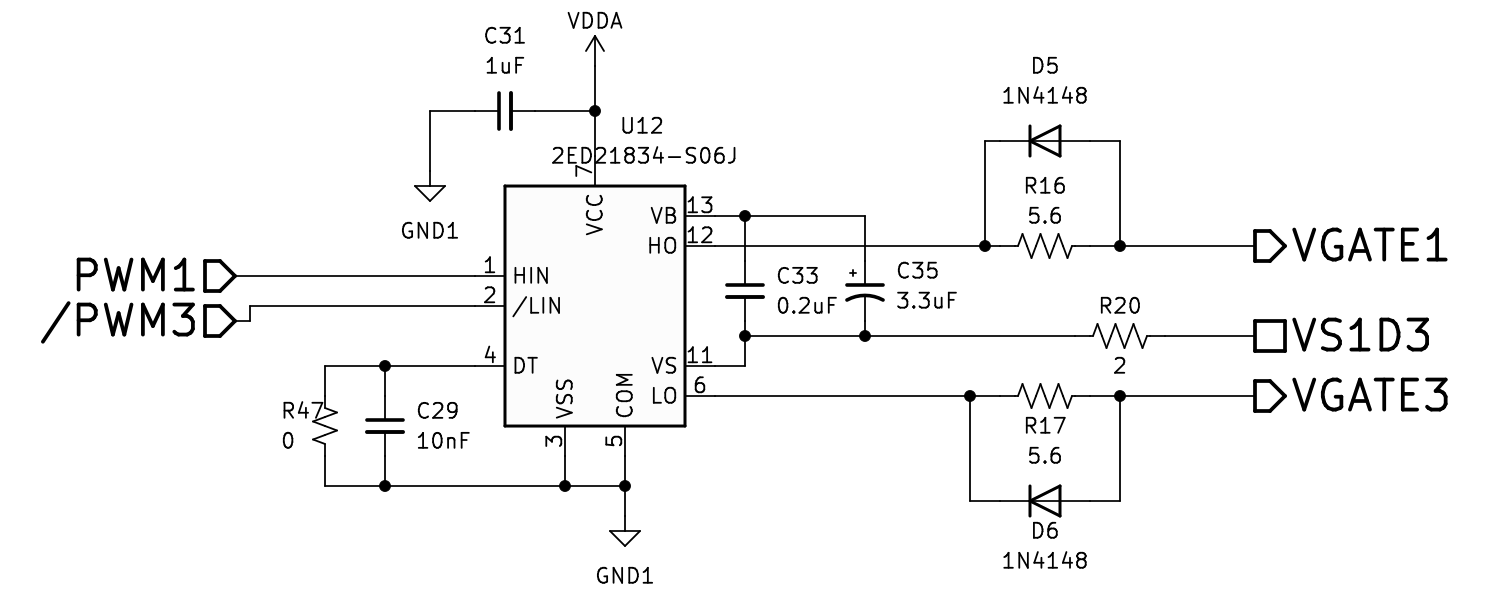
\includegraphics[scale=0.95]{Imagenes/Circuito Driver.png}
    \caption{Circuito de conexión del driver 2ED21834-S06J. El circuito del driver para la otra columna es idéntico.}
    \label{circuito_driver}
\end{figure}

Aquí se puede ver el driver, indicado por la referencia U12, al que le llegan las señales de comando PWM a sus pines HIN y /LIN para el transistor del lado alto y bajo de la columna respectivamente (al estar negada  la entrada para el transistor bajo, la señal que le llega debe estar invertida). Luego, conectado entre el pin DT y tierra se encuentra la resistencia de dead-time, que cuyo valor define el dead-time o tiempo muerto $t_{DT}$. En la salida, se conecta a los pines HO (alto) y LO (bajo) una resistencia limitadora en paralelo con un diodo que permite la descarga de las capacitancias de los transistores, y entre los pines VB y VS se coloca el capacitor que completa el circuito de bootstrap, que se explicará mas adelante. En lo que hace referencia a conexiones a tierra, este circuito, al estar del lado primario del convertidor, se conecta a la referencia $GND_1$. Según la hoja de datos, la tensión de alimentación debe ser de entre \SI[]{10}[]{\volt} y \SI[]{20}[]{\volt}, por lo que se alimenta con una tensión no regulada de \num{12}-\SI[]{18}[]{\volt}.\\

El dimensionamiento de todos estos componentes se va a tratar a continuación siguiendo las recomendaciones del fabricante disponibles en hojas de datos y notas.

\subsubsection{Dimensionamiento de Componentes}

\lipsum[1]\\

\lipsum[2]\\

\subsubsection{Esquema Interno del Dispositivo}

{\Bold\scshape Falta completar esta sección.}\\

\lipsum[1]\\

\begin{figure}[h]
    \centering
    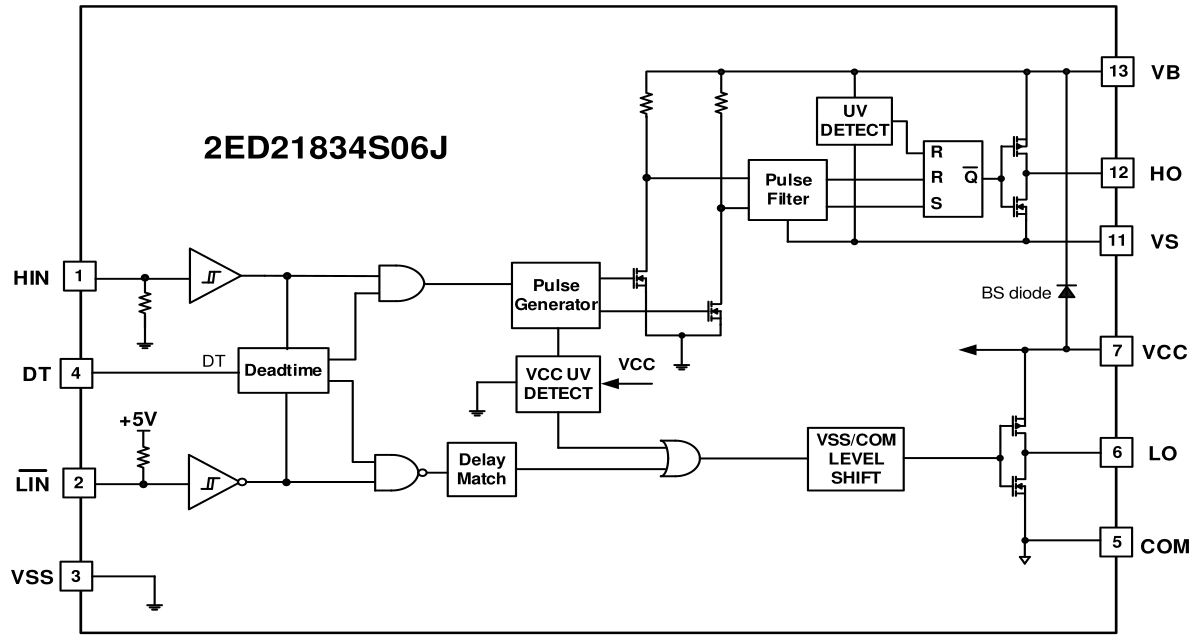
\includegraphics[scale=0.25]{Imagenes/Esquema Interno Driver.png}
    \caption{Diagrama de bloques interno del driver 2ED21834-S06J de Infineon Technologies.}
    \label{interno_driver}
\end{figure}

\lipsum[2]\\

\lipsum[3]\\

\lipsum[4]\\

\newpage

\input{Secciones/3 - Diseno de la Plataforma/3.4 - Sistema de Medición.tex}

\newpage

\subsection{Etapa de Aislación de Señal}

Ahora se debe implementar un circuito auxiliar que provea una aislación galvánica entre los componentes que se sitúan del lado de potencia de la plataforma (como los transistores, diodos, circuito driver, etc.), y los componentes de la parte digital del sistema (como el controlador digital de señales, el circuito de acondicionamiento, etc.).\\

Existen tres partes principales de la plataforma, donde se pasa de la parte digital a la de potencia, donde se requiere algún tipo de aislación:\\

\begin{enumerate}
    \item Entre las salidas PWM del controlador y las entradas de comando de los drivers 2ED21834-S06J de la figura \ref{circuito_driver}.
    \item Para las líneas del bus I\textsuperscript{2}C que comunican al sensor LM5056A de la figura \ref{conexion_LM5056A} (lado de potencia) con el módulo I\textsuperscript{2}C del controlador.
    \item Para la medición de corriente de salida mediante el sensor de efecto Hall TMCS1100A4 de la figura \ref{conexion_TMCS1100}.
    \item Para generar fuentes de alimentación aisladas para los circuitos del lado digital.\\
\end{enumerate}

En este capítulo vamos a tratar las soluciones de aislación para los primeros dos casos. En el tercer caso, el TMCS1100A4, al ser un dispositivo que funciona por medio del efecto Hall, ya tiene aislación incluida en su diseño, por lo que la salida del mismo ya se encuentra aislada del convertidor. Para el cuarto ítem, esto se va a tratar propiamente y en profundidad en la sección de este capítulo dedicada a los circuitos de alimentación de la plataforma.\\

\subsubsection{Tecnologías de Aislación de Señal}

{\Bold\scshape Falta completar esta sección.}\\

\lipsum[1]\\

\subsubsection{Aislación de los Drivers}

Cómo los drivers están conectados directamente a terminales de los transistores de potencia del convertidor, estos se encuentran dentro de la etapa de potencia de la plataforma. Sin embargo, las señales PWM que definen el tiempo y secuencia de conmutación de los transistores provienen del módulo PWM del controlador digital, todo dentro del área digital de la plataforma. Entonces, previo a las entradas de señal de los 2ED21834-S06J se debe interponer algun circuito de aislación de señal, para mantener la separación entre potencia y señal.\\

\lipsum[2]\\

\subsubsection{Aislación I\textsuperscript{2}C}

\lipsum[2]\\



\newpage

\subsection{Sistema de Control}

{\Large\Bold\scshape Falta completar esta sección.}\\

\lipsum[1]\\

\lipsum[2]\\

\newpage

\subsection{Circuito de Alimentación}

\lipsum[3]\\

\lipsum[4]\\